\chapter{User Interface Design}

\section{Complex Transaction Form}

\subsection{Registration Form (for \texttt{staff})}

\begin{figure}[h]
	\centerline
	{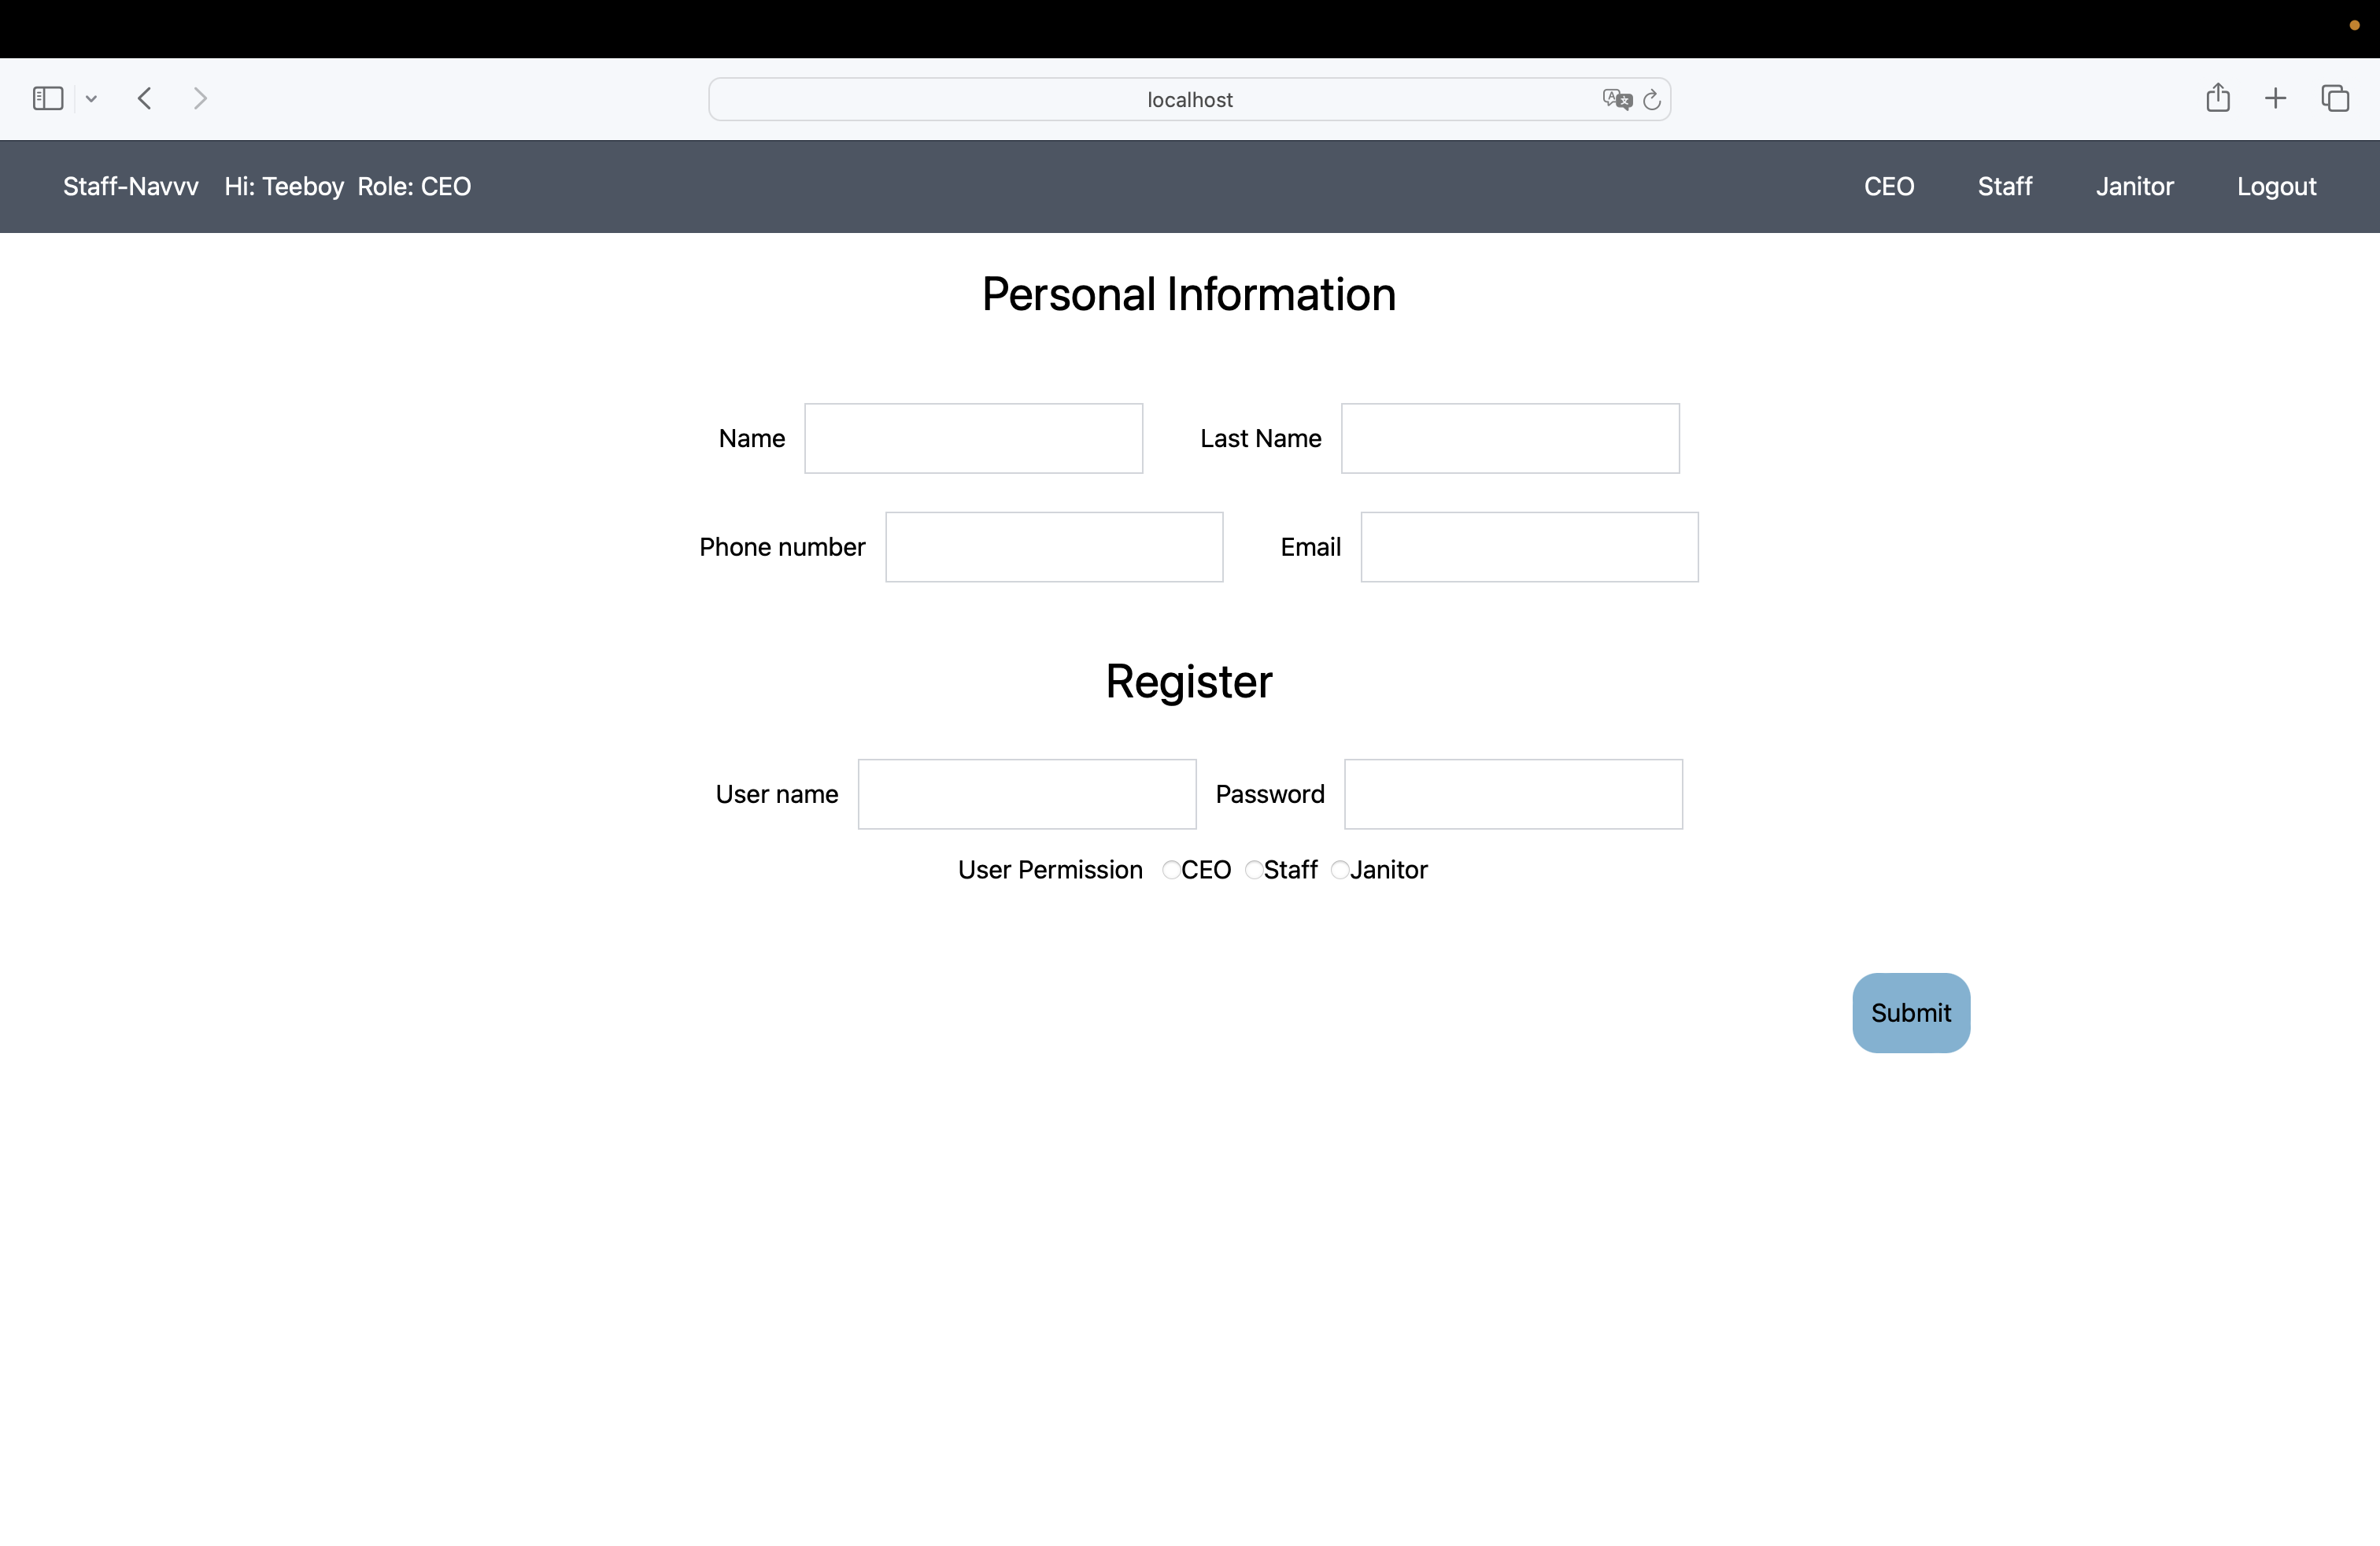
\includegraphics[width=12cm]{fig/2_register}}
	%{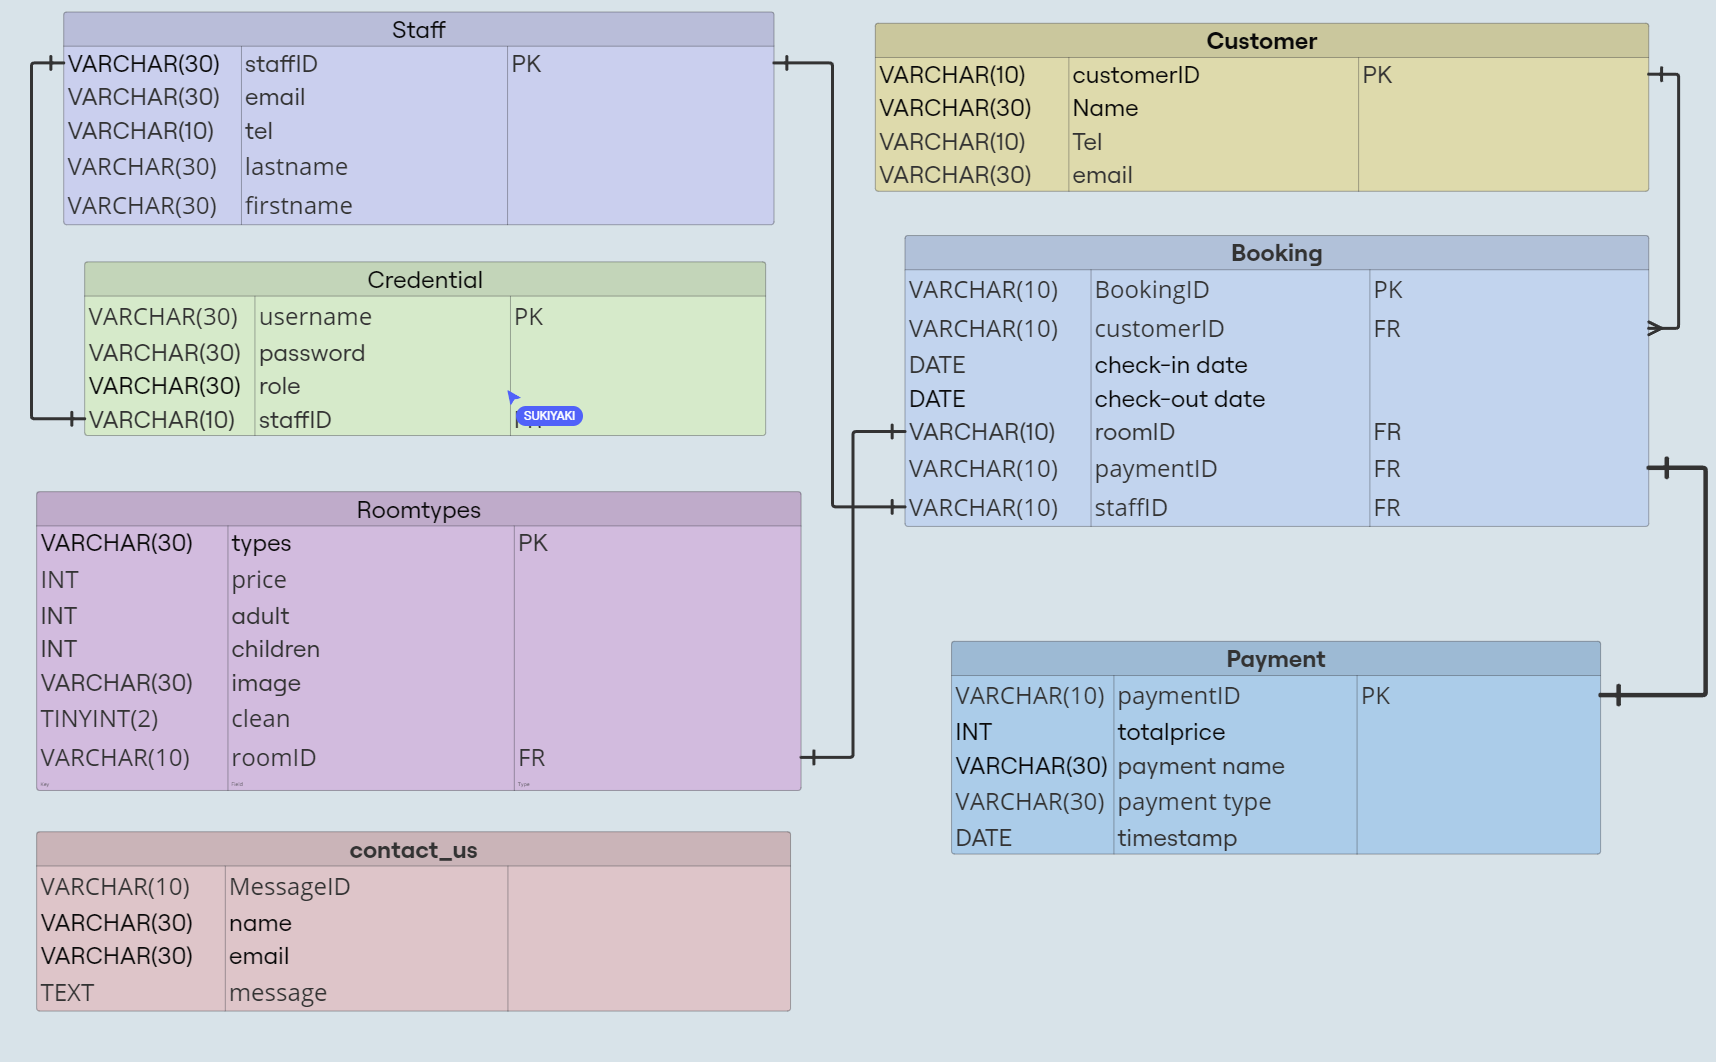
\includegraphics[]{fig/ERD_v1}}
	\caption{Registration form}
\end{figure} 

It is capable of creating both staff and users through the same UI. 

Relations involved is based on guest or staff:

\begin{description}
	\item[Set 1] Guest only
	\item[Set 2] Staff, Position, Ground, Manager
\end{description}

\subsection{Booking form (for \texttt{user})}

\begin{figure}[h]
	\centerline
	{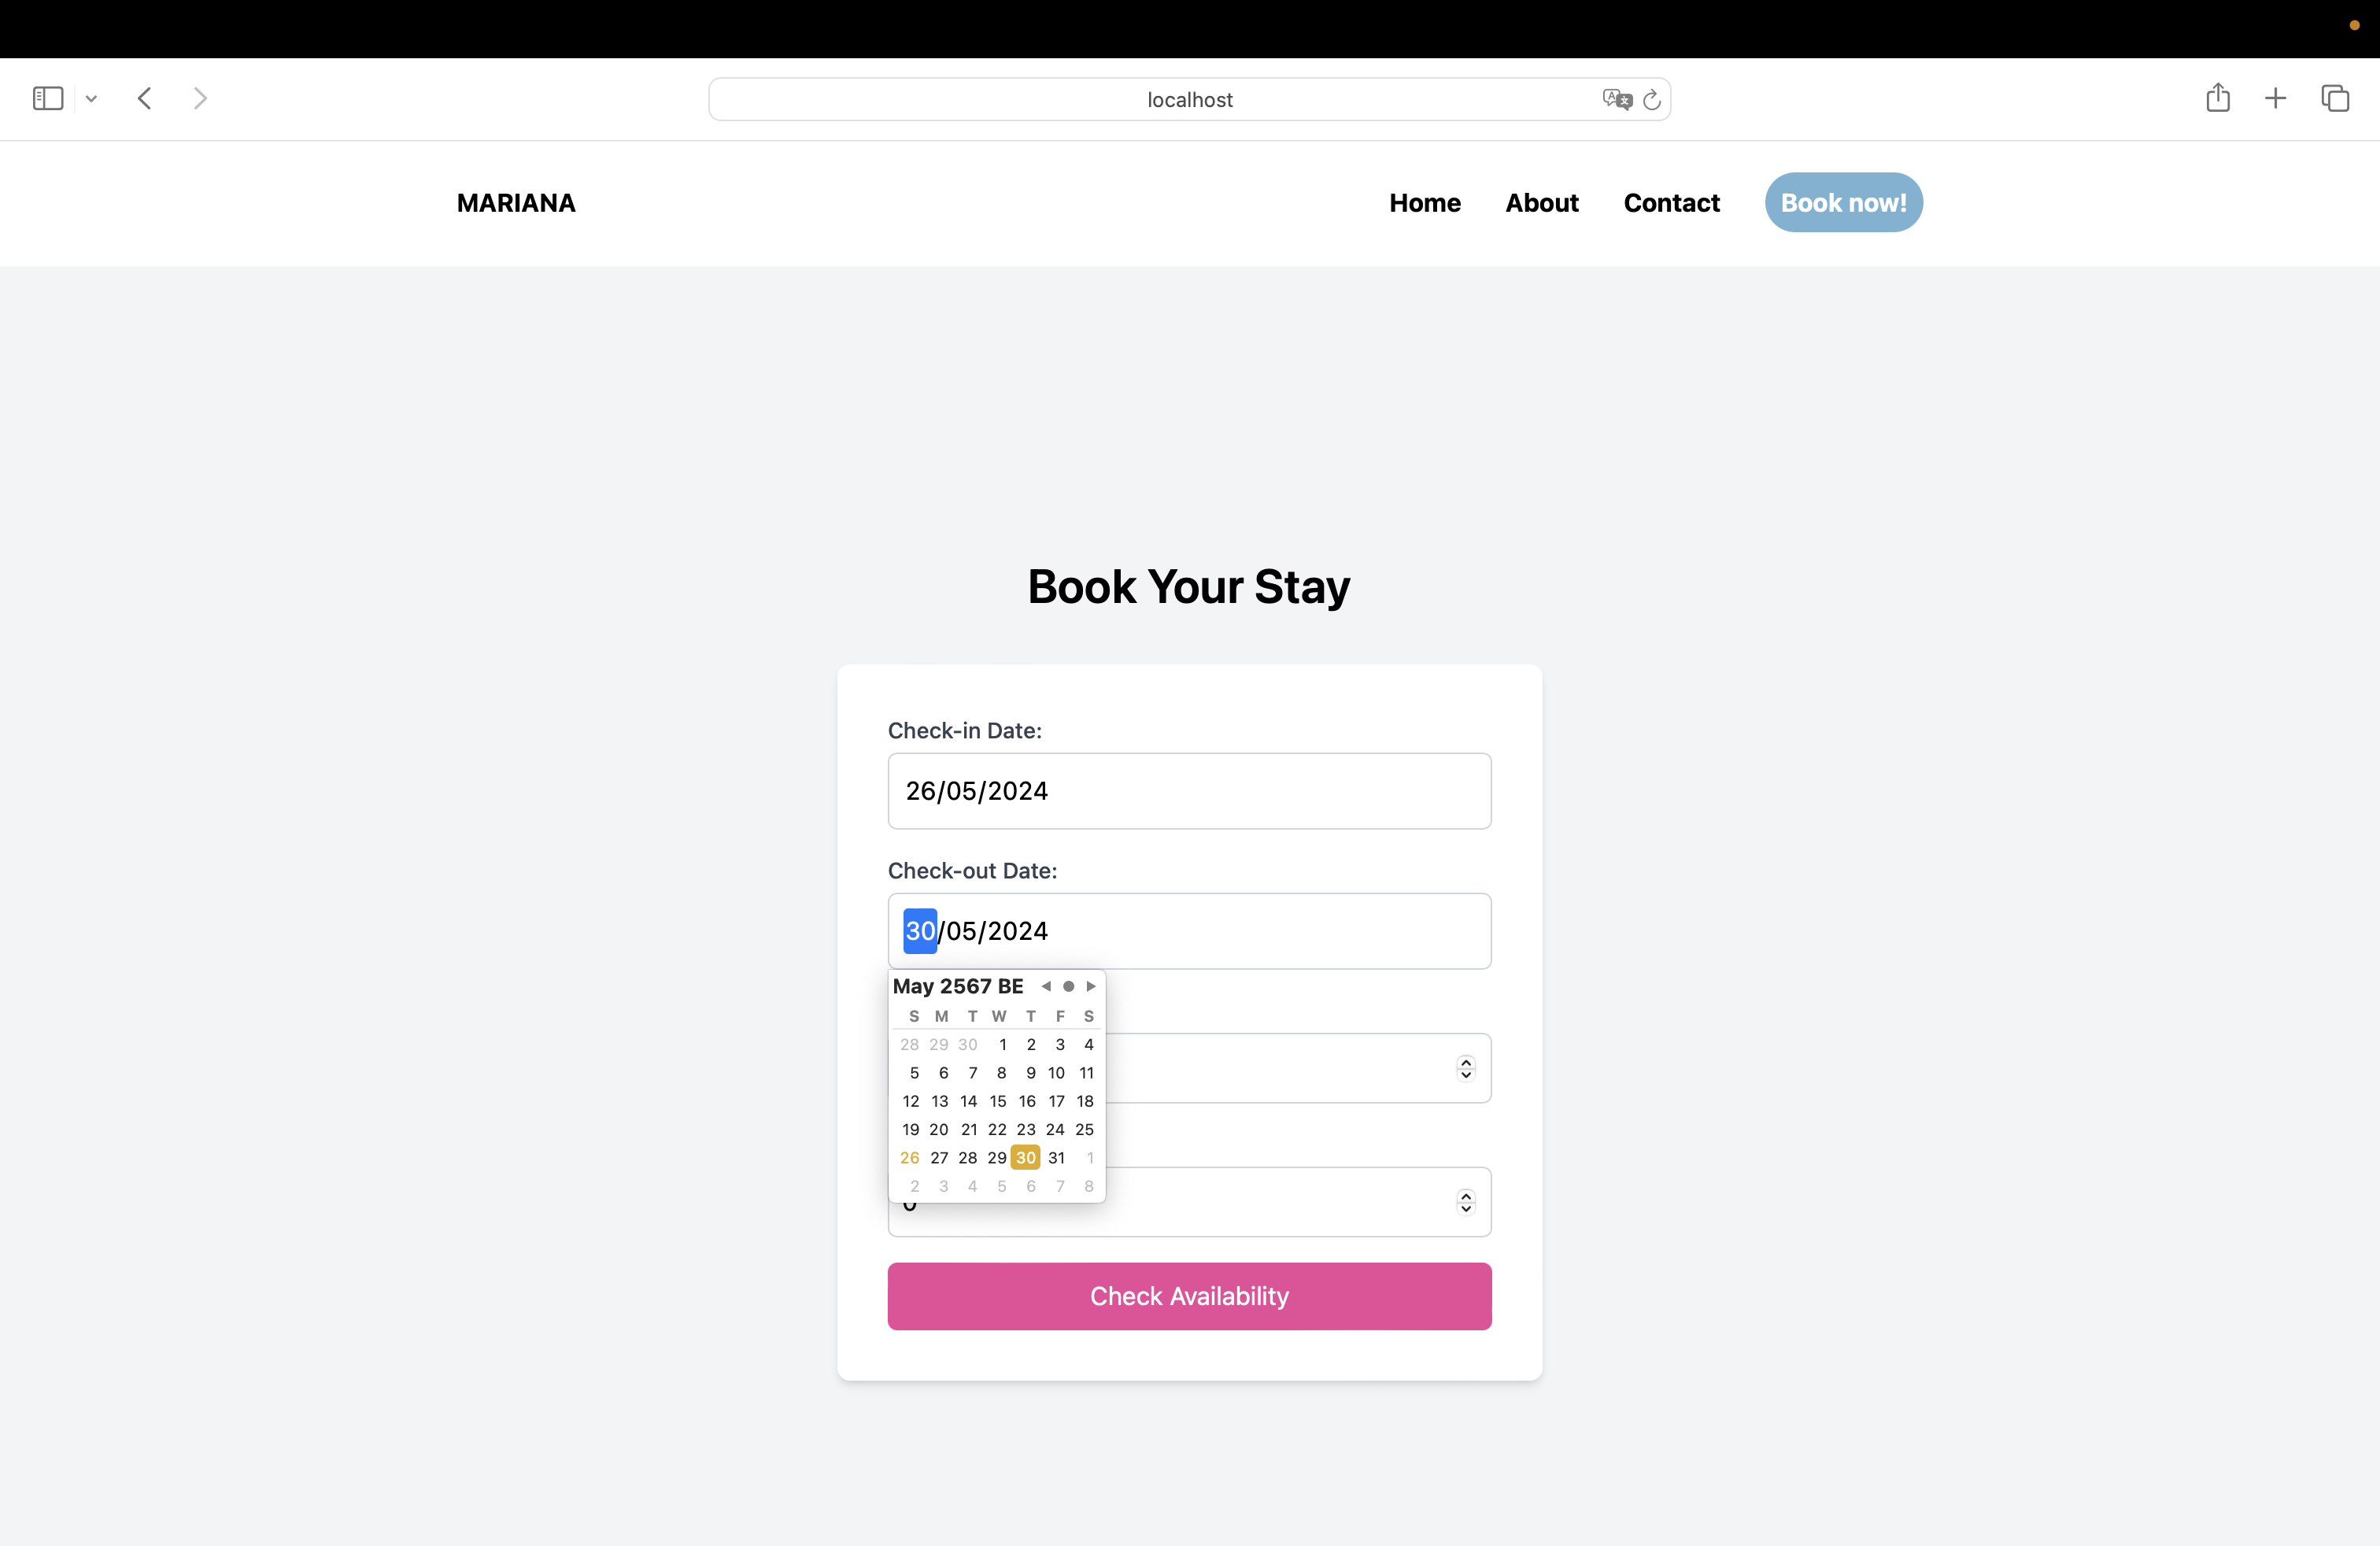
\includegraphics[width=12cm]{fig/4_book}}
	%{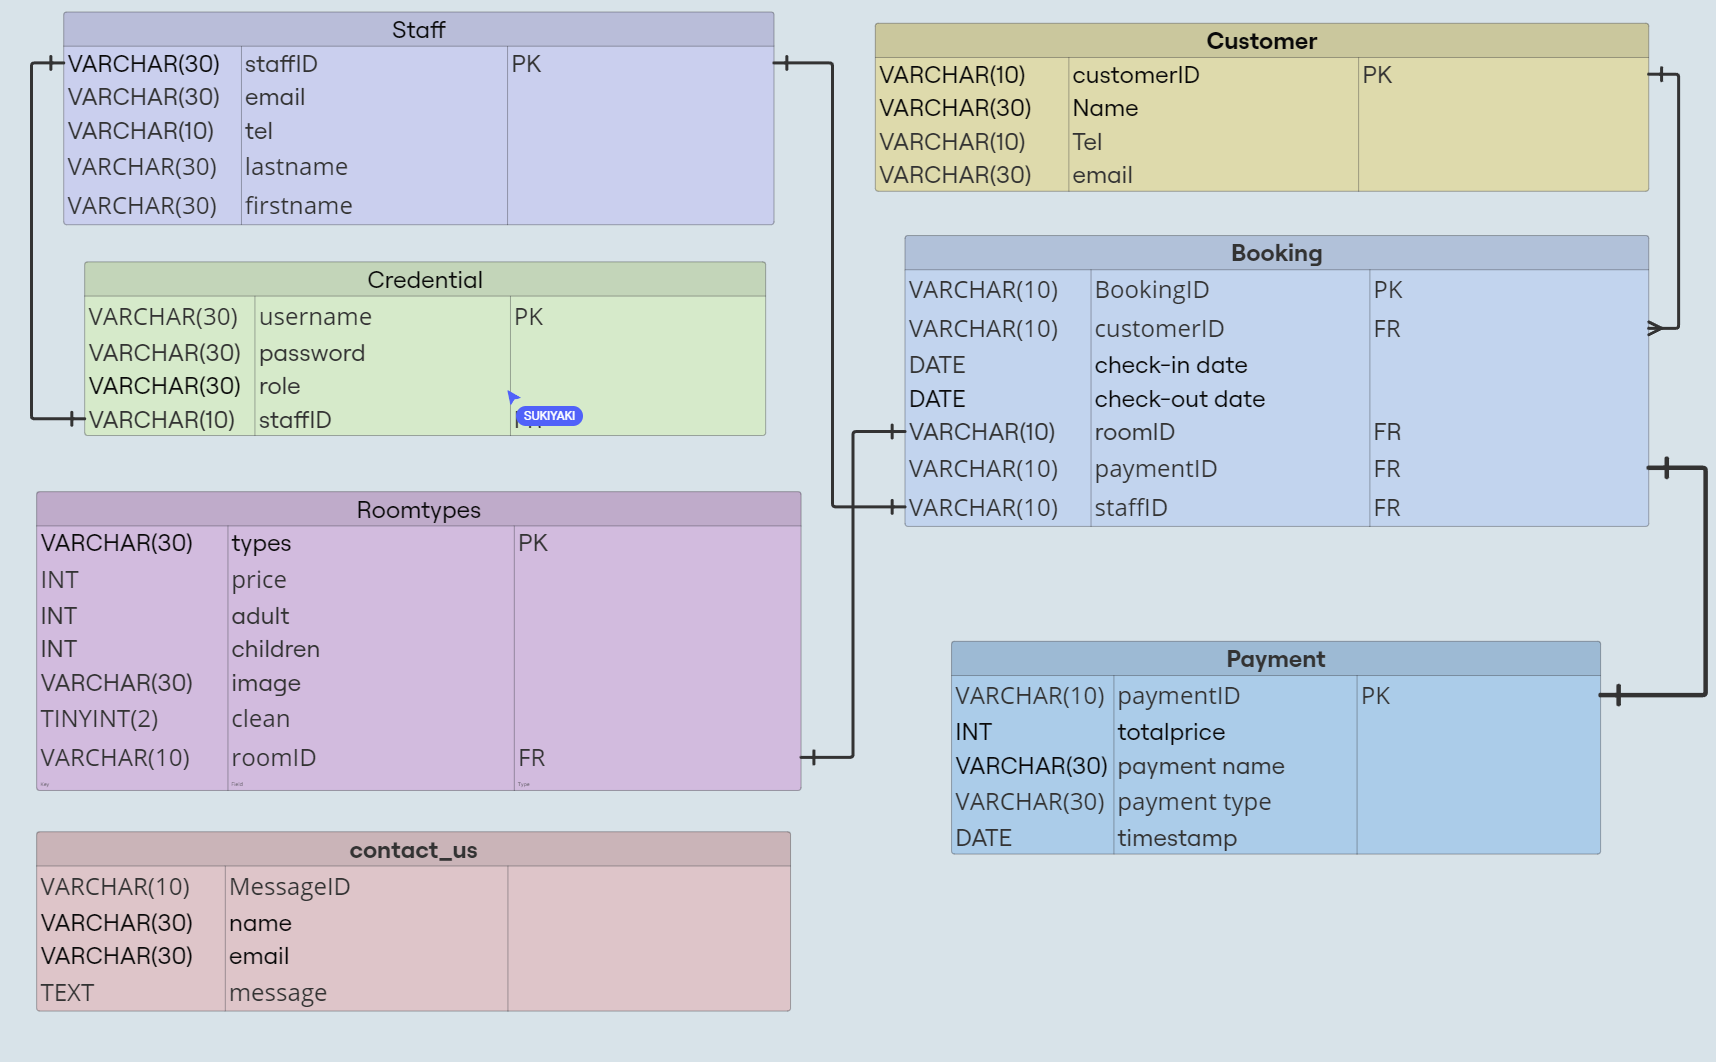
\includegraphics[]{fig/ERD_v1}}
	\caption{Booking form}
\end{figure}

Relations involved: Reservations, Service, GuestInfo

\subsection{Housekeeping form}

\begin{figure}[h]
	\centerline
	{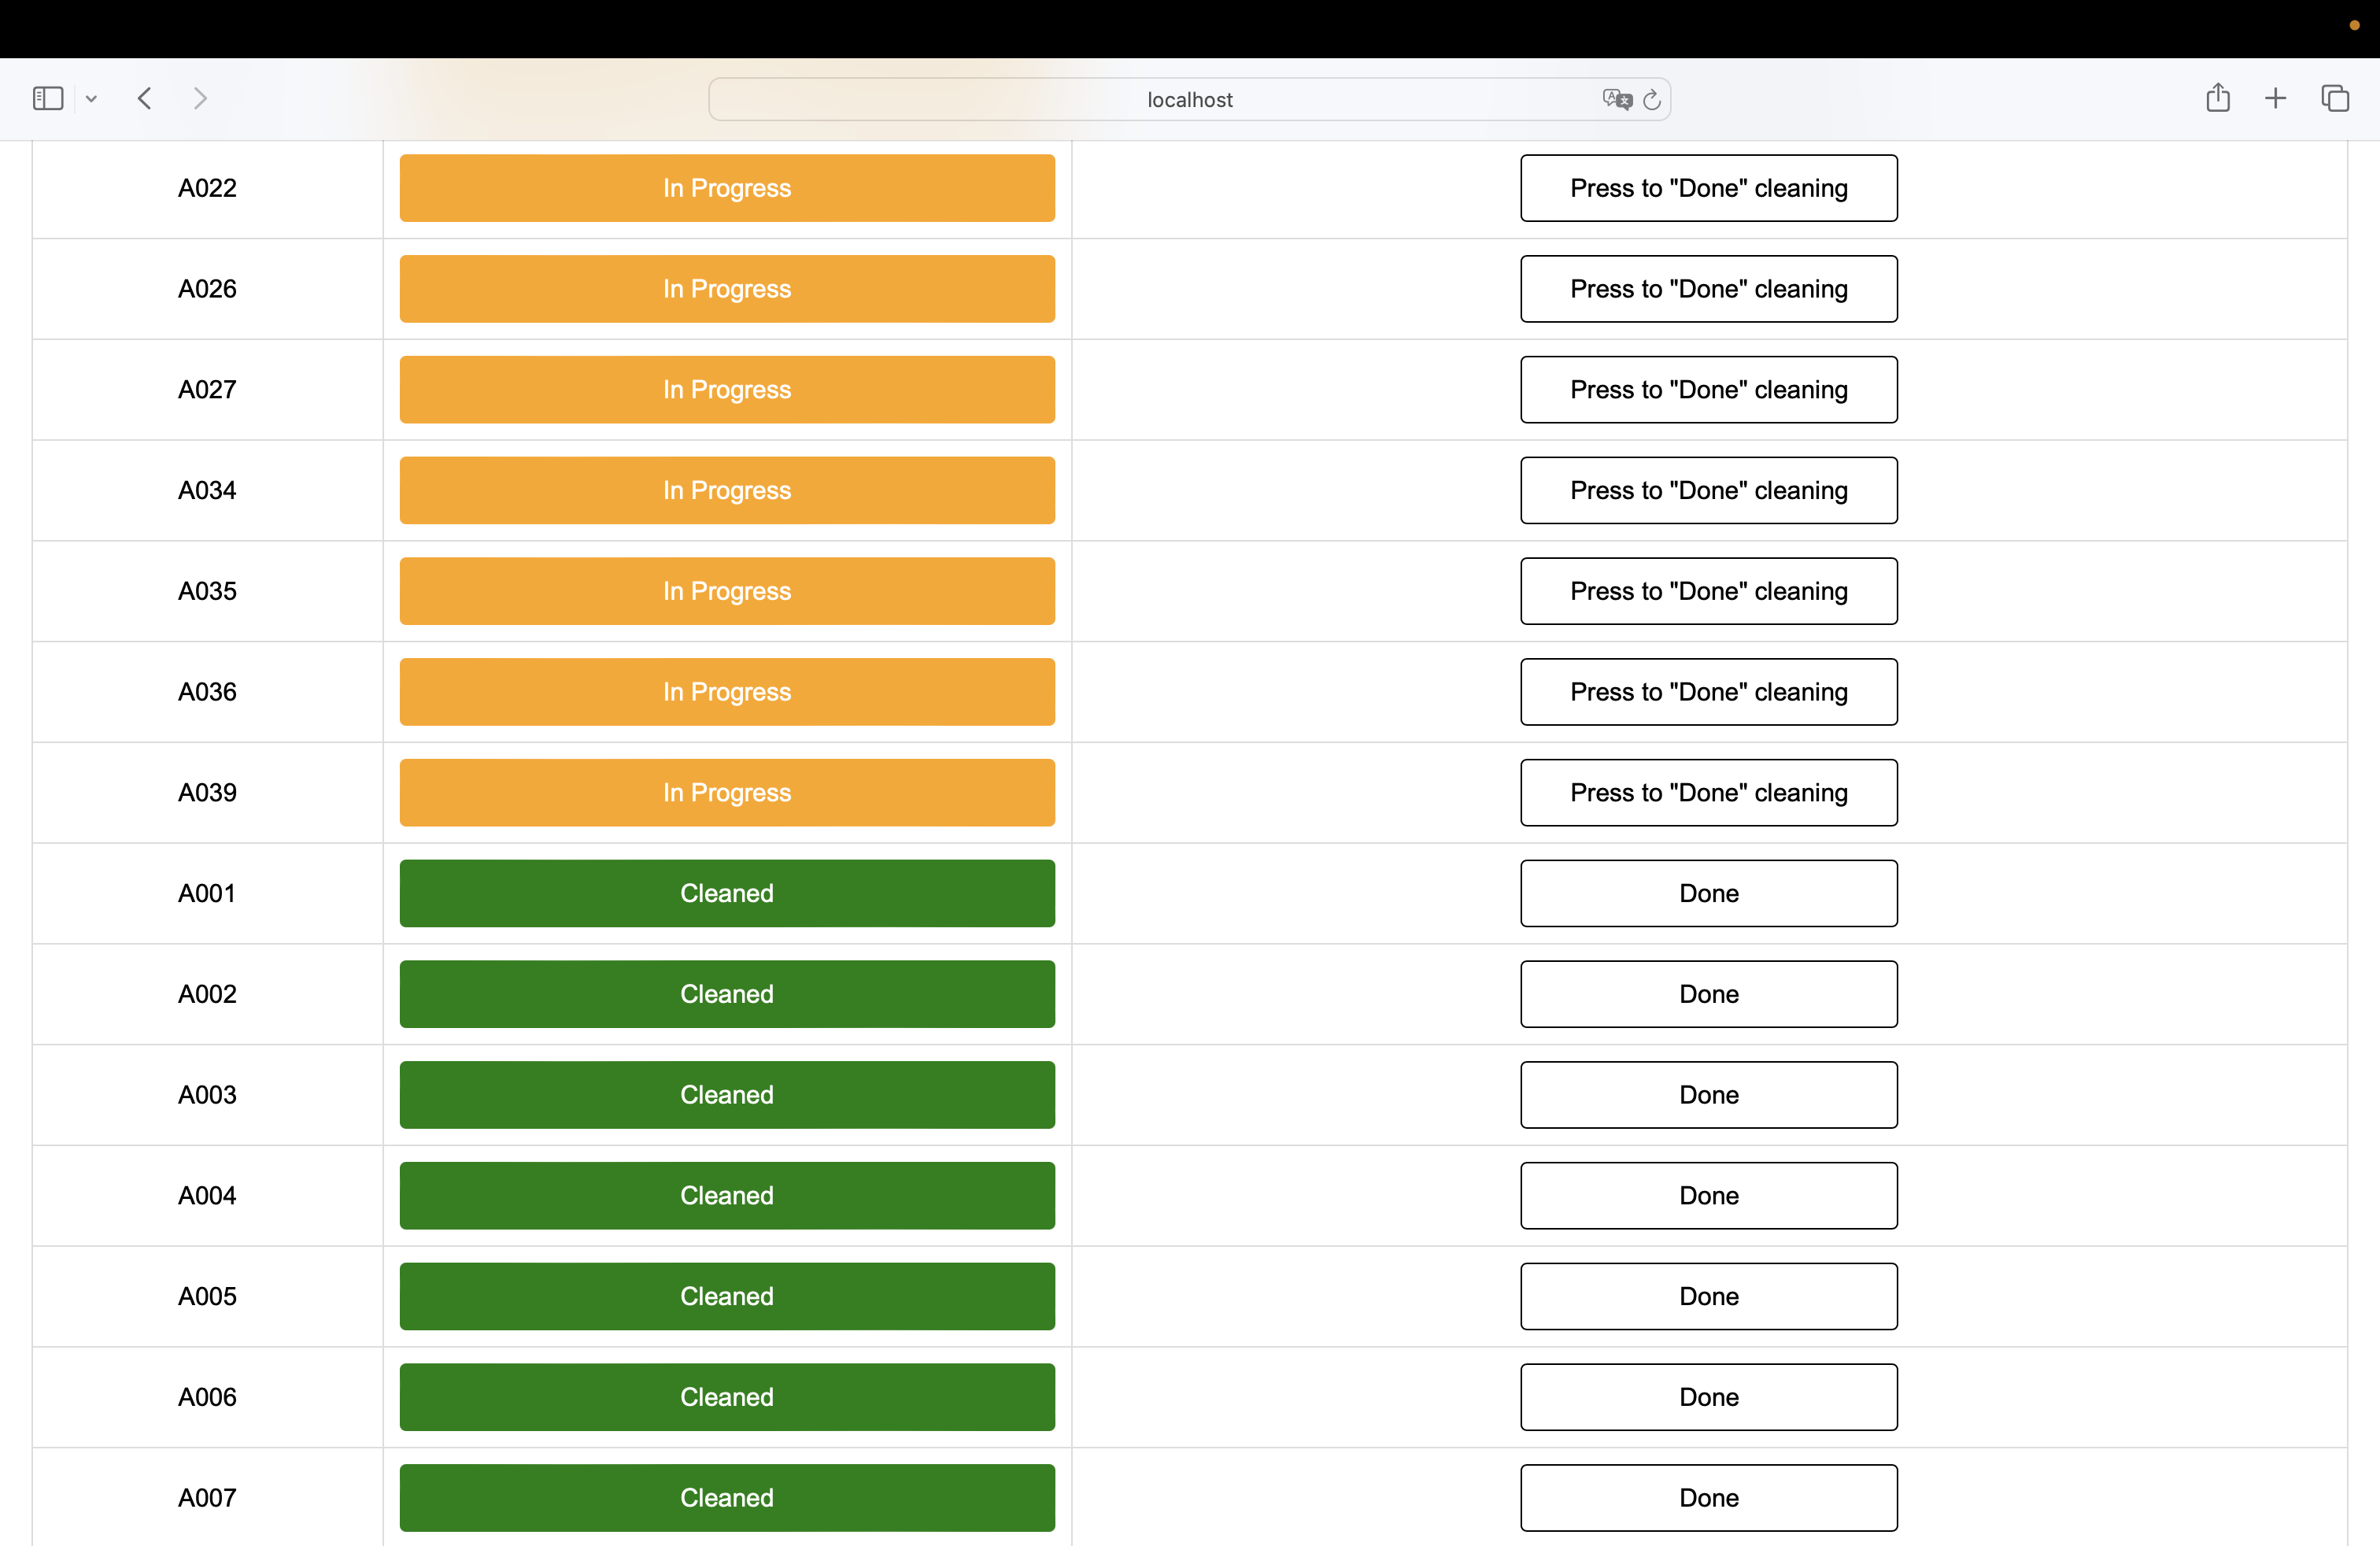
\includegraphics[width=12cm]{fig/1_house}}
	%{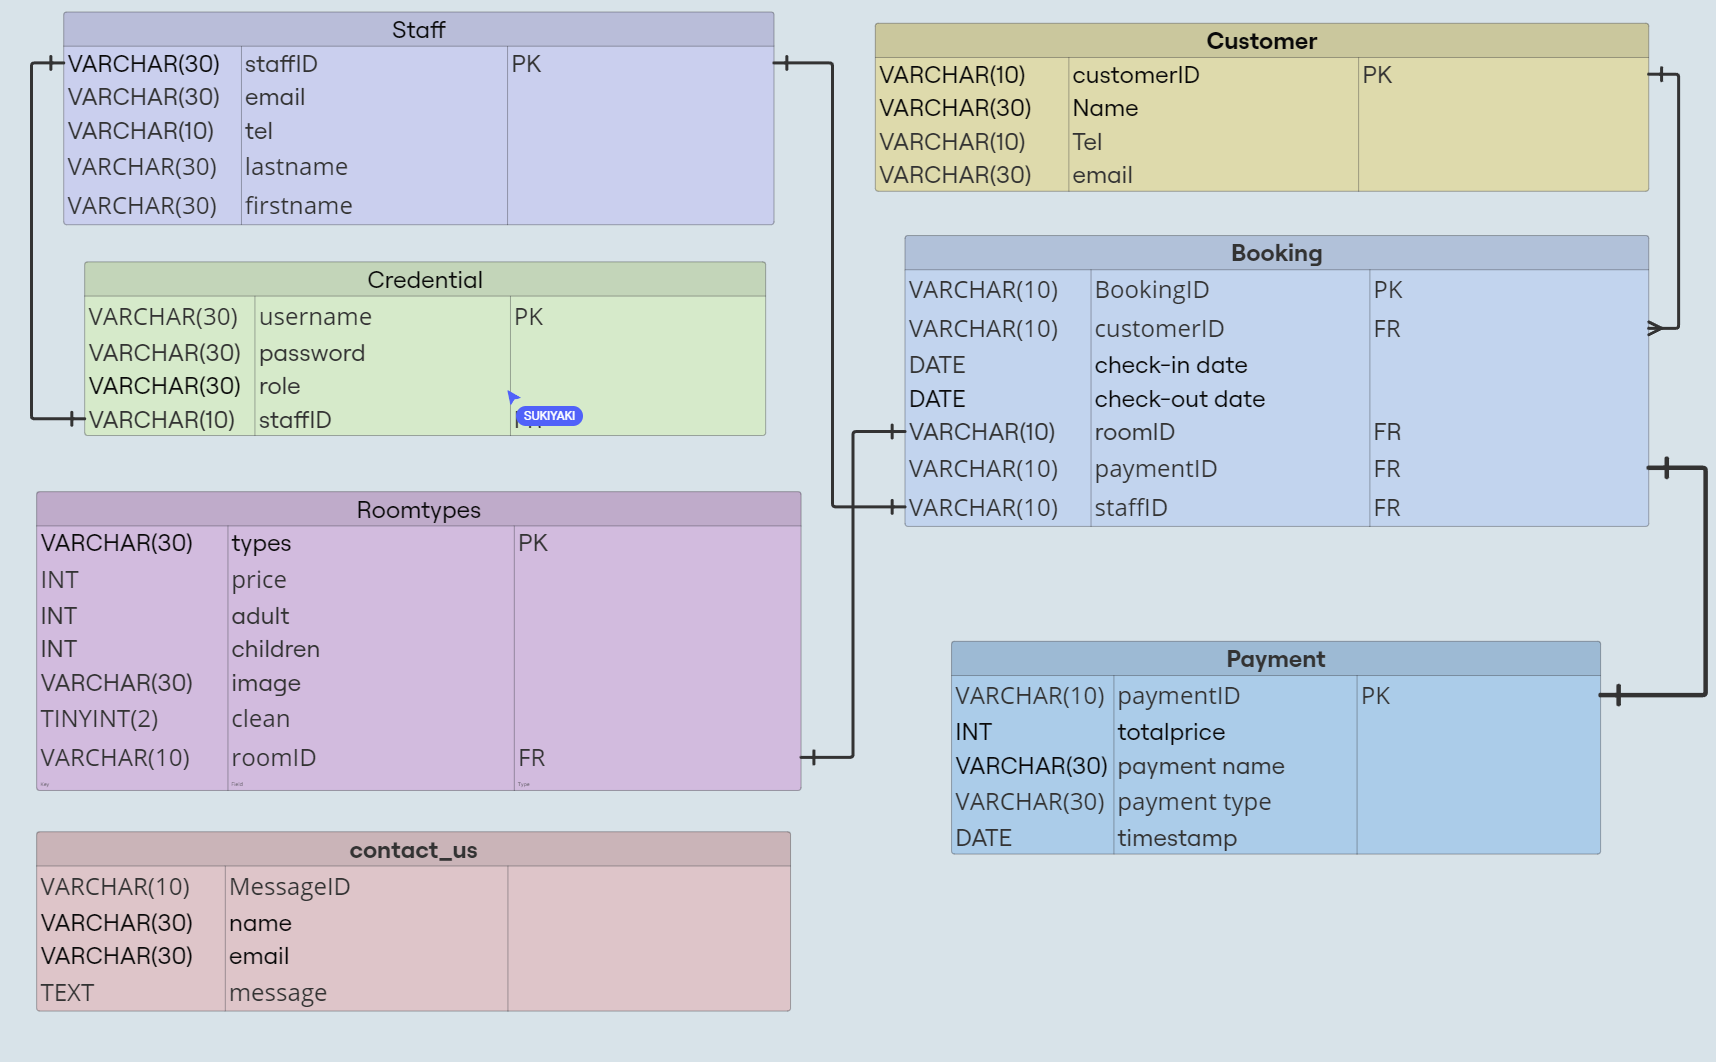
\includegraphics[]{fig/ERD_v1}}
	\caption{Housekeeping form}
\end{figure} 

The housekeeping form also serves bidirectionally as a report.

Relations involved: Ground, Management, Ground Task Info, Ground Task Tickets

\subsection{Room form}

\begin{figure}[h]
	\centerline
	{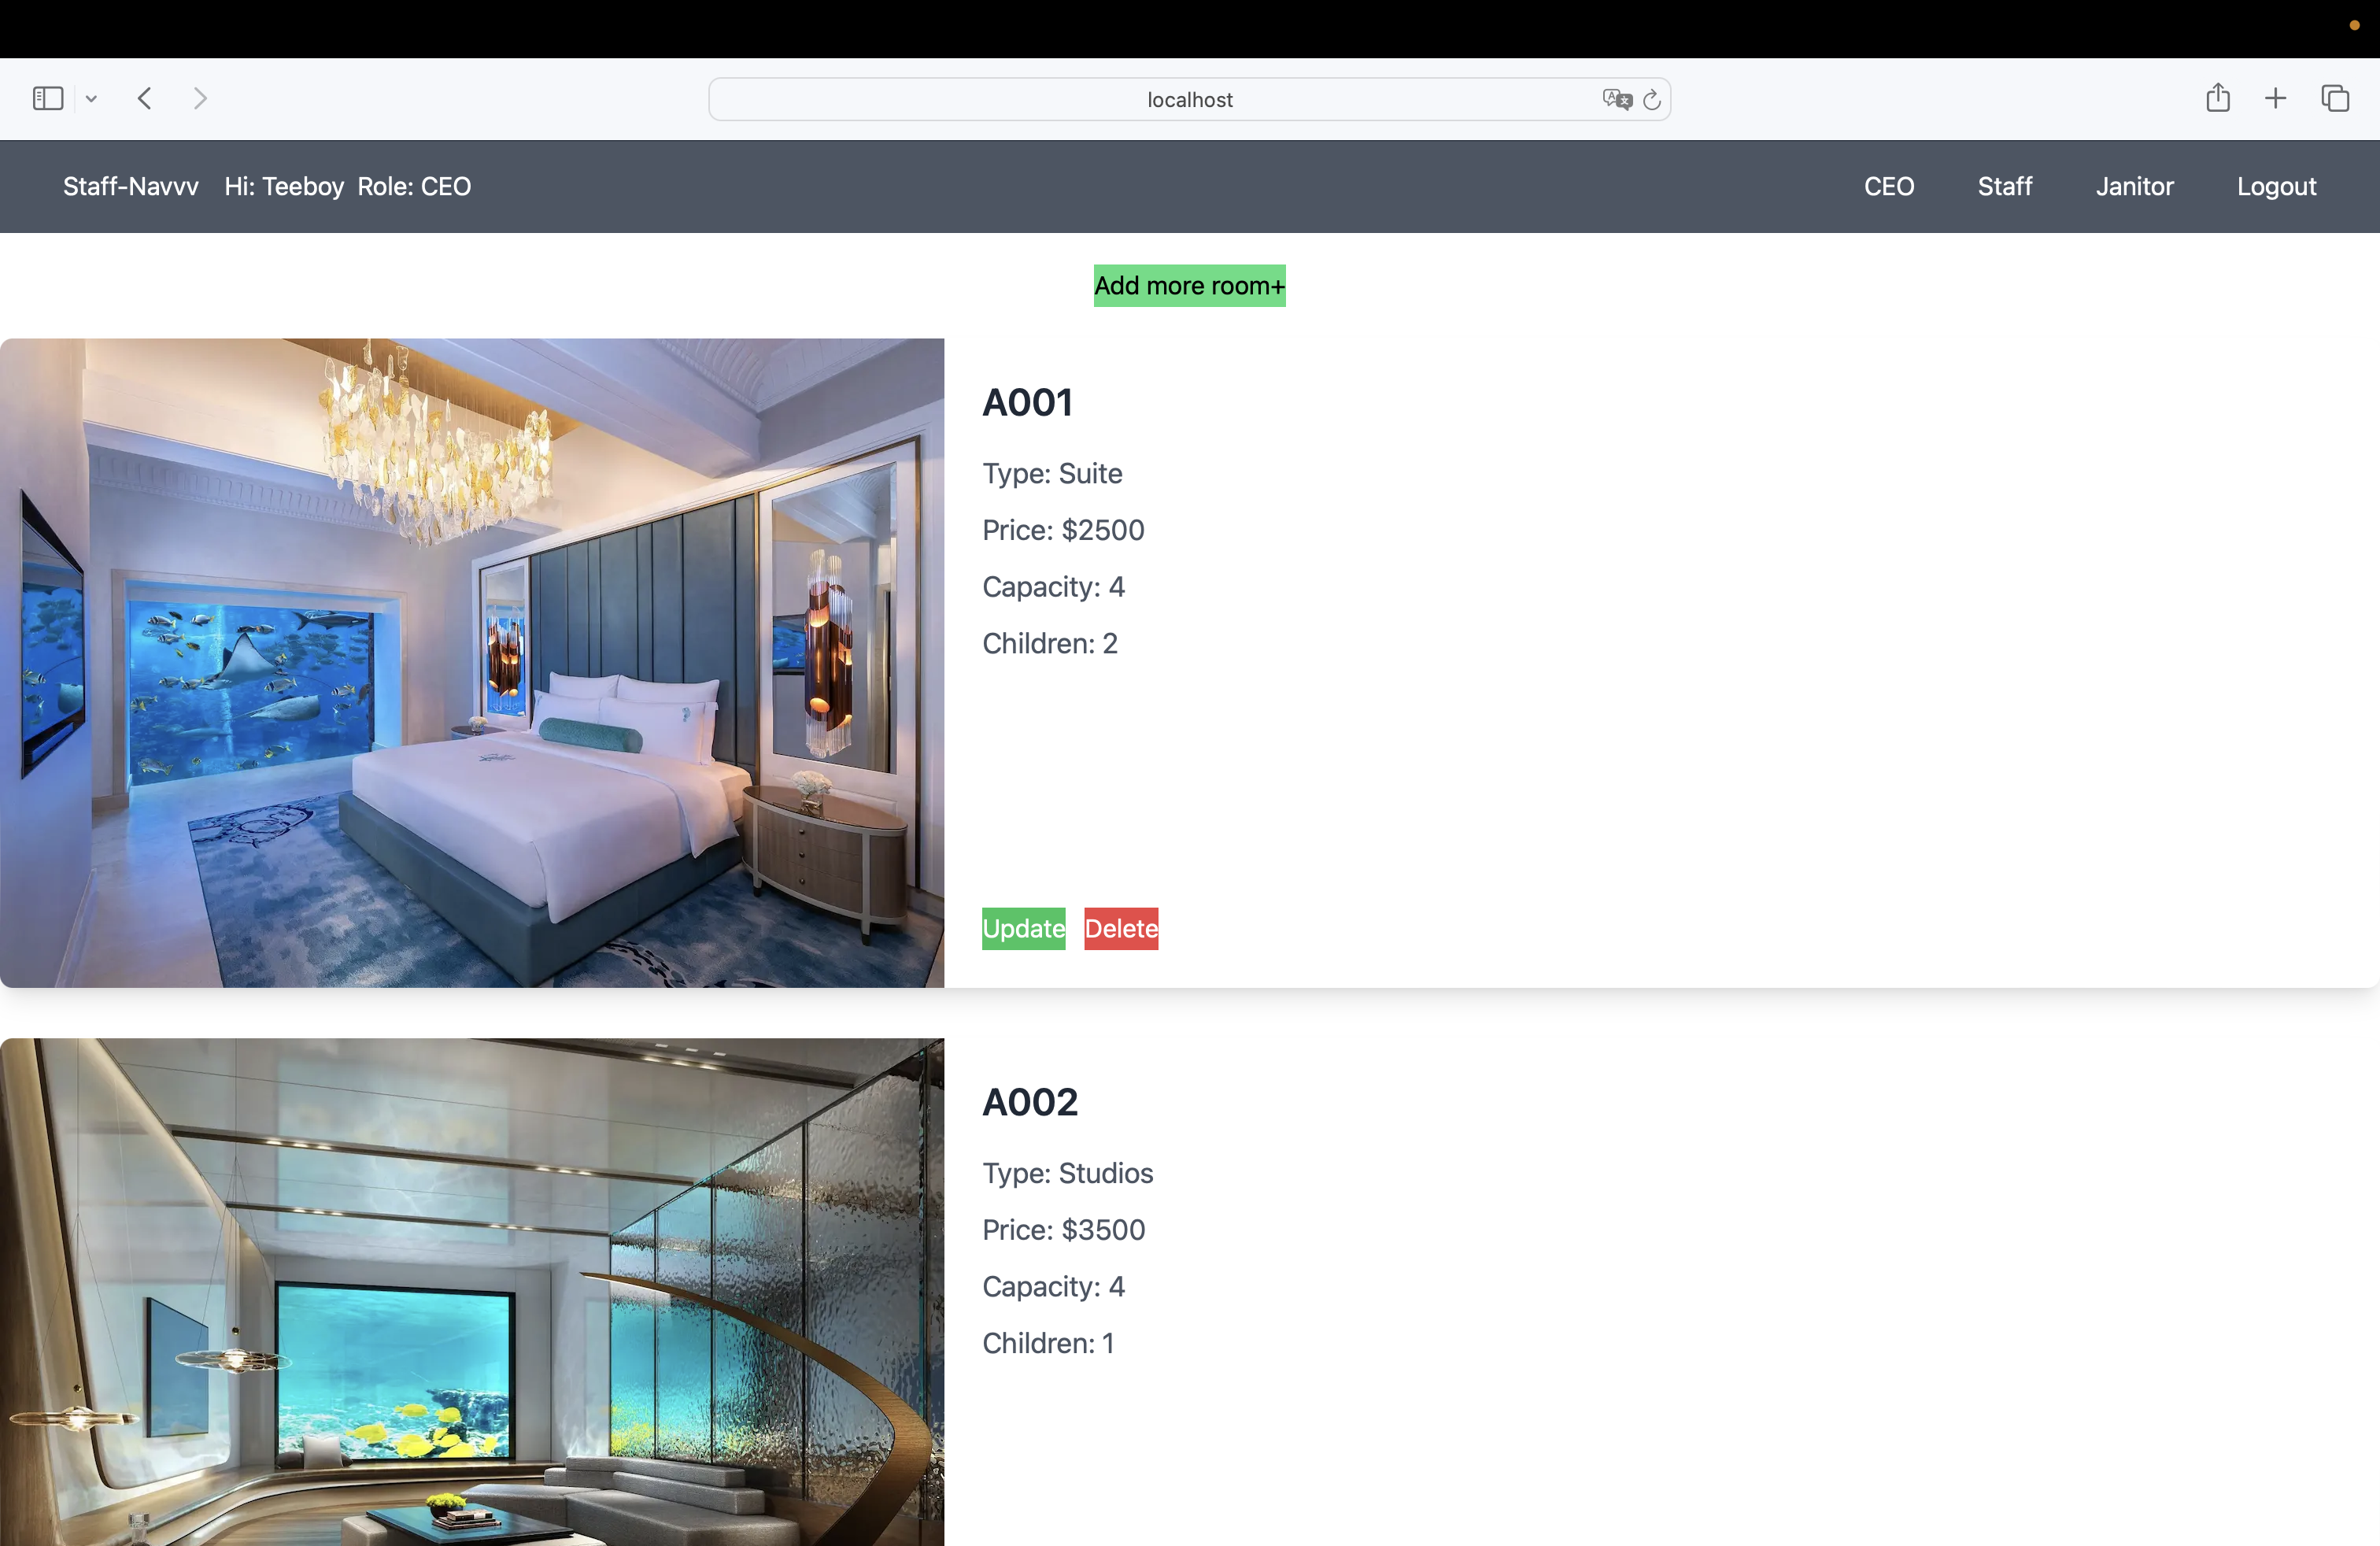
\includegraphics[width=12cm]{fig/3_rooms}}
	%{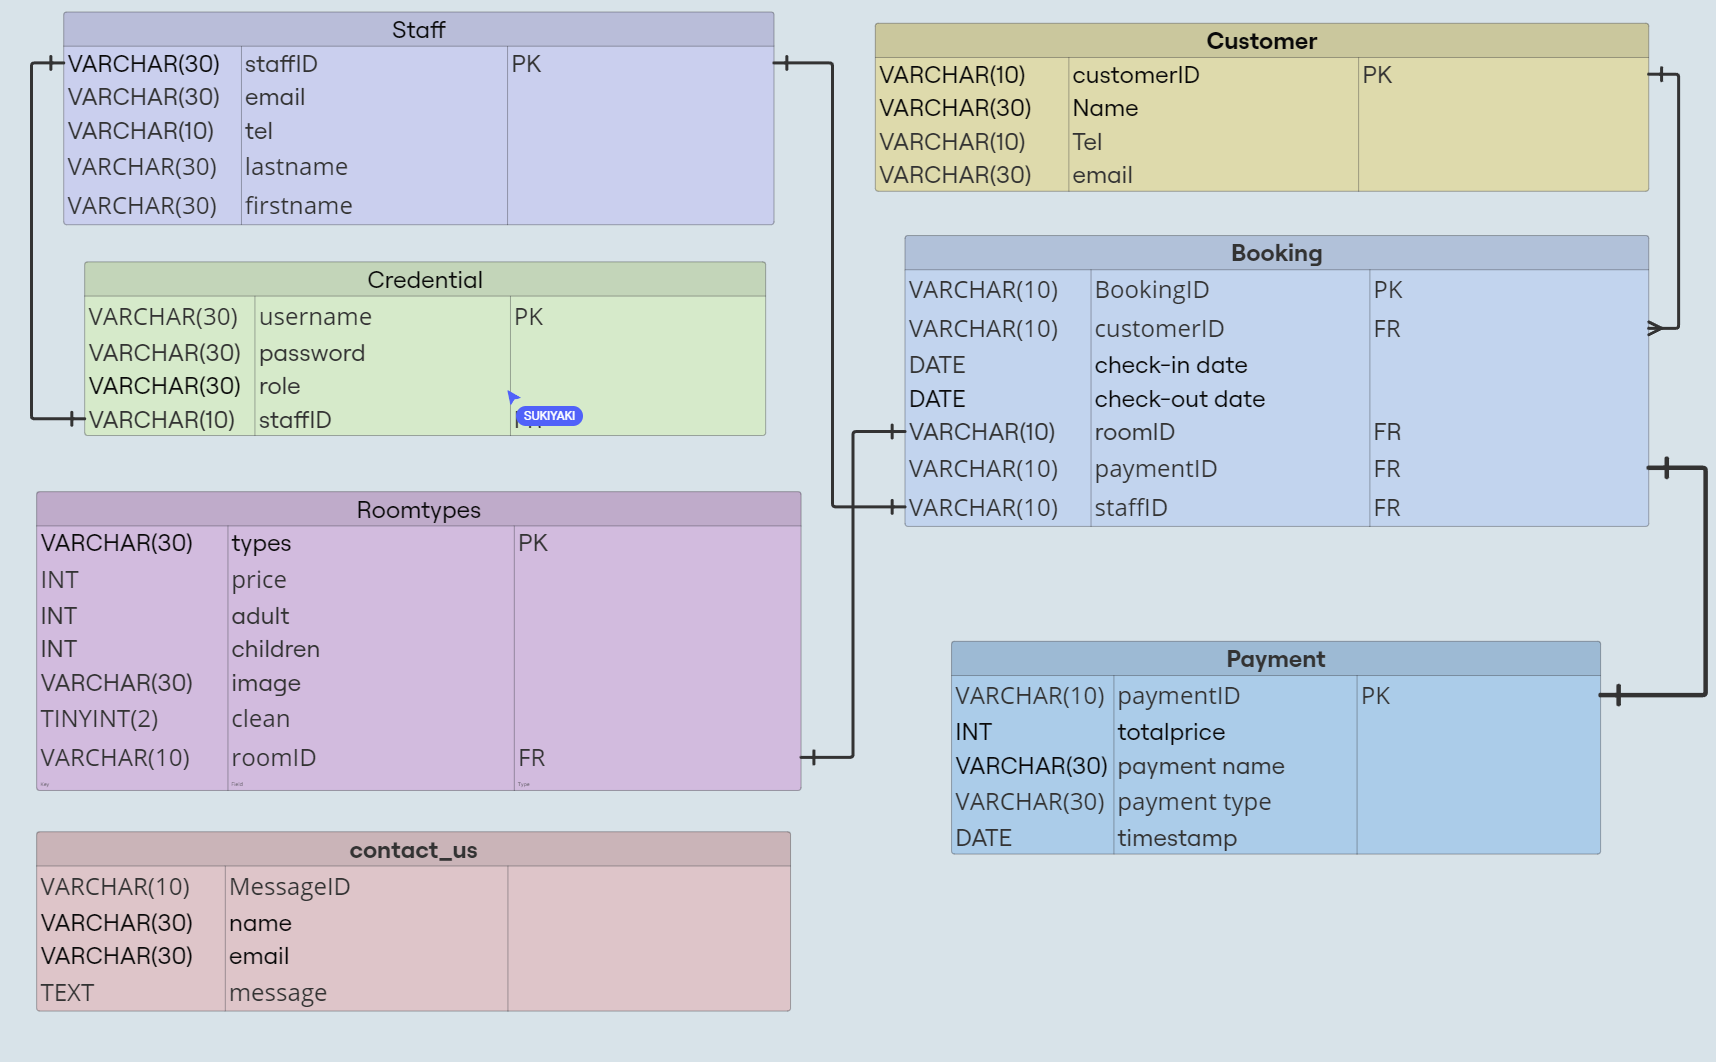
\includegraphics[]{fig/ERD_v1}}
	\caption{Room form}
\end{figure} 

Relations involved: Facility, Property, Service

\section{Advanced Analysis Report}

\subsection{Summary Report}
\begin{figure}[h]
	\centerline
	{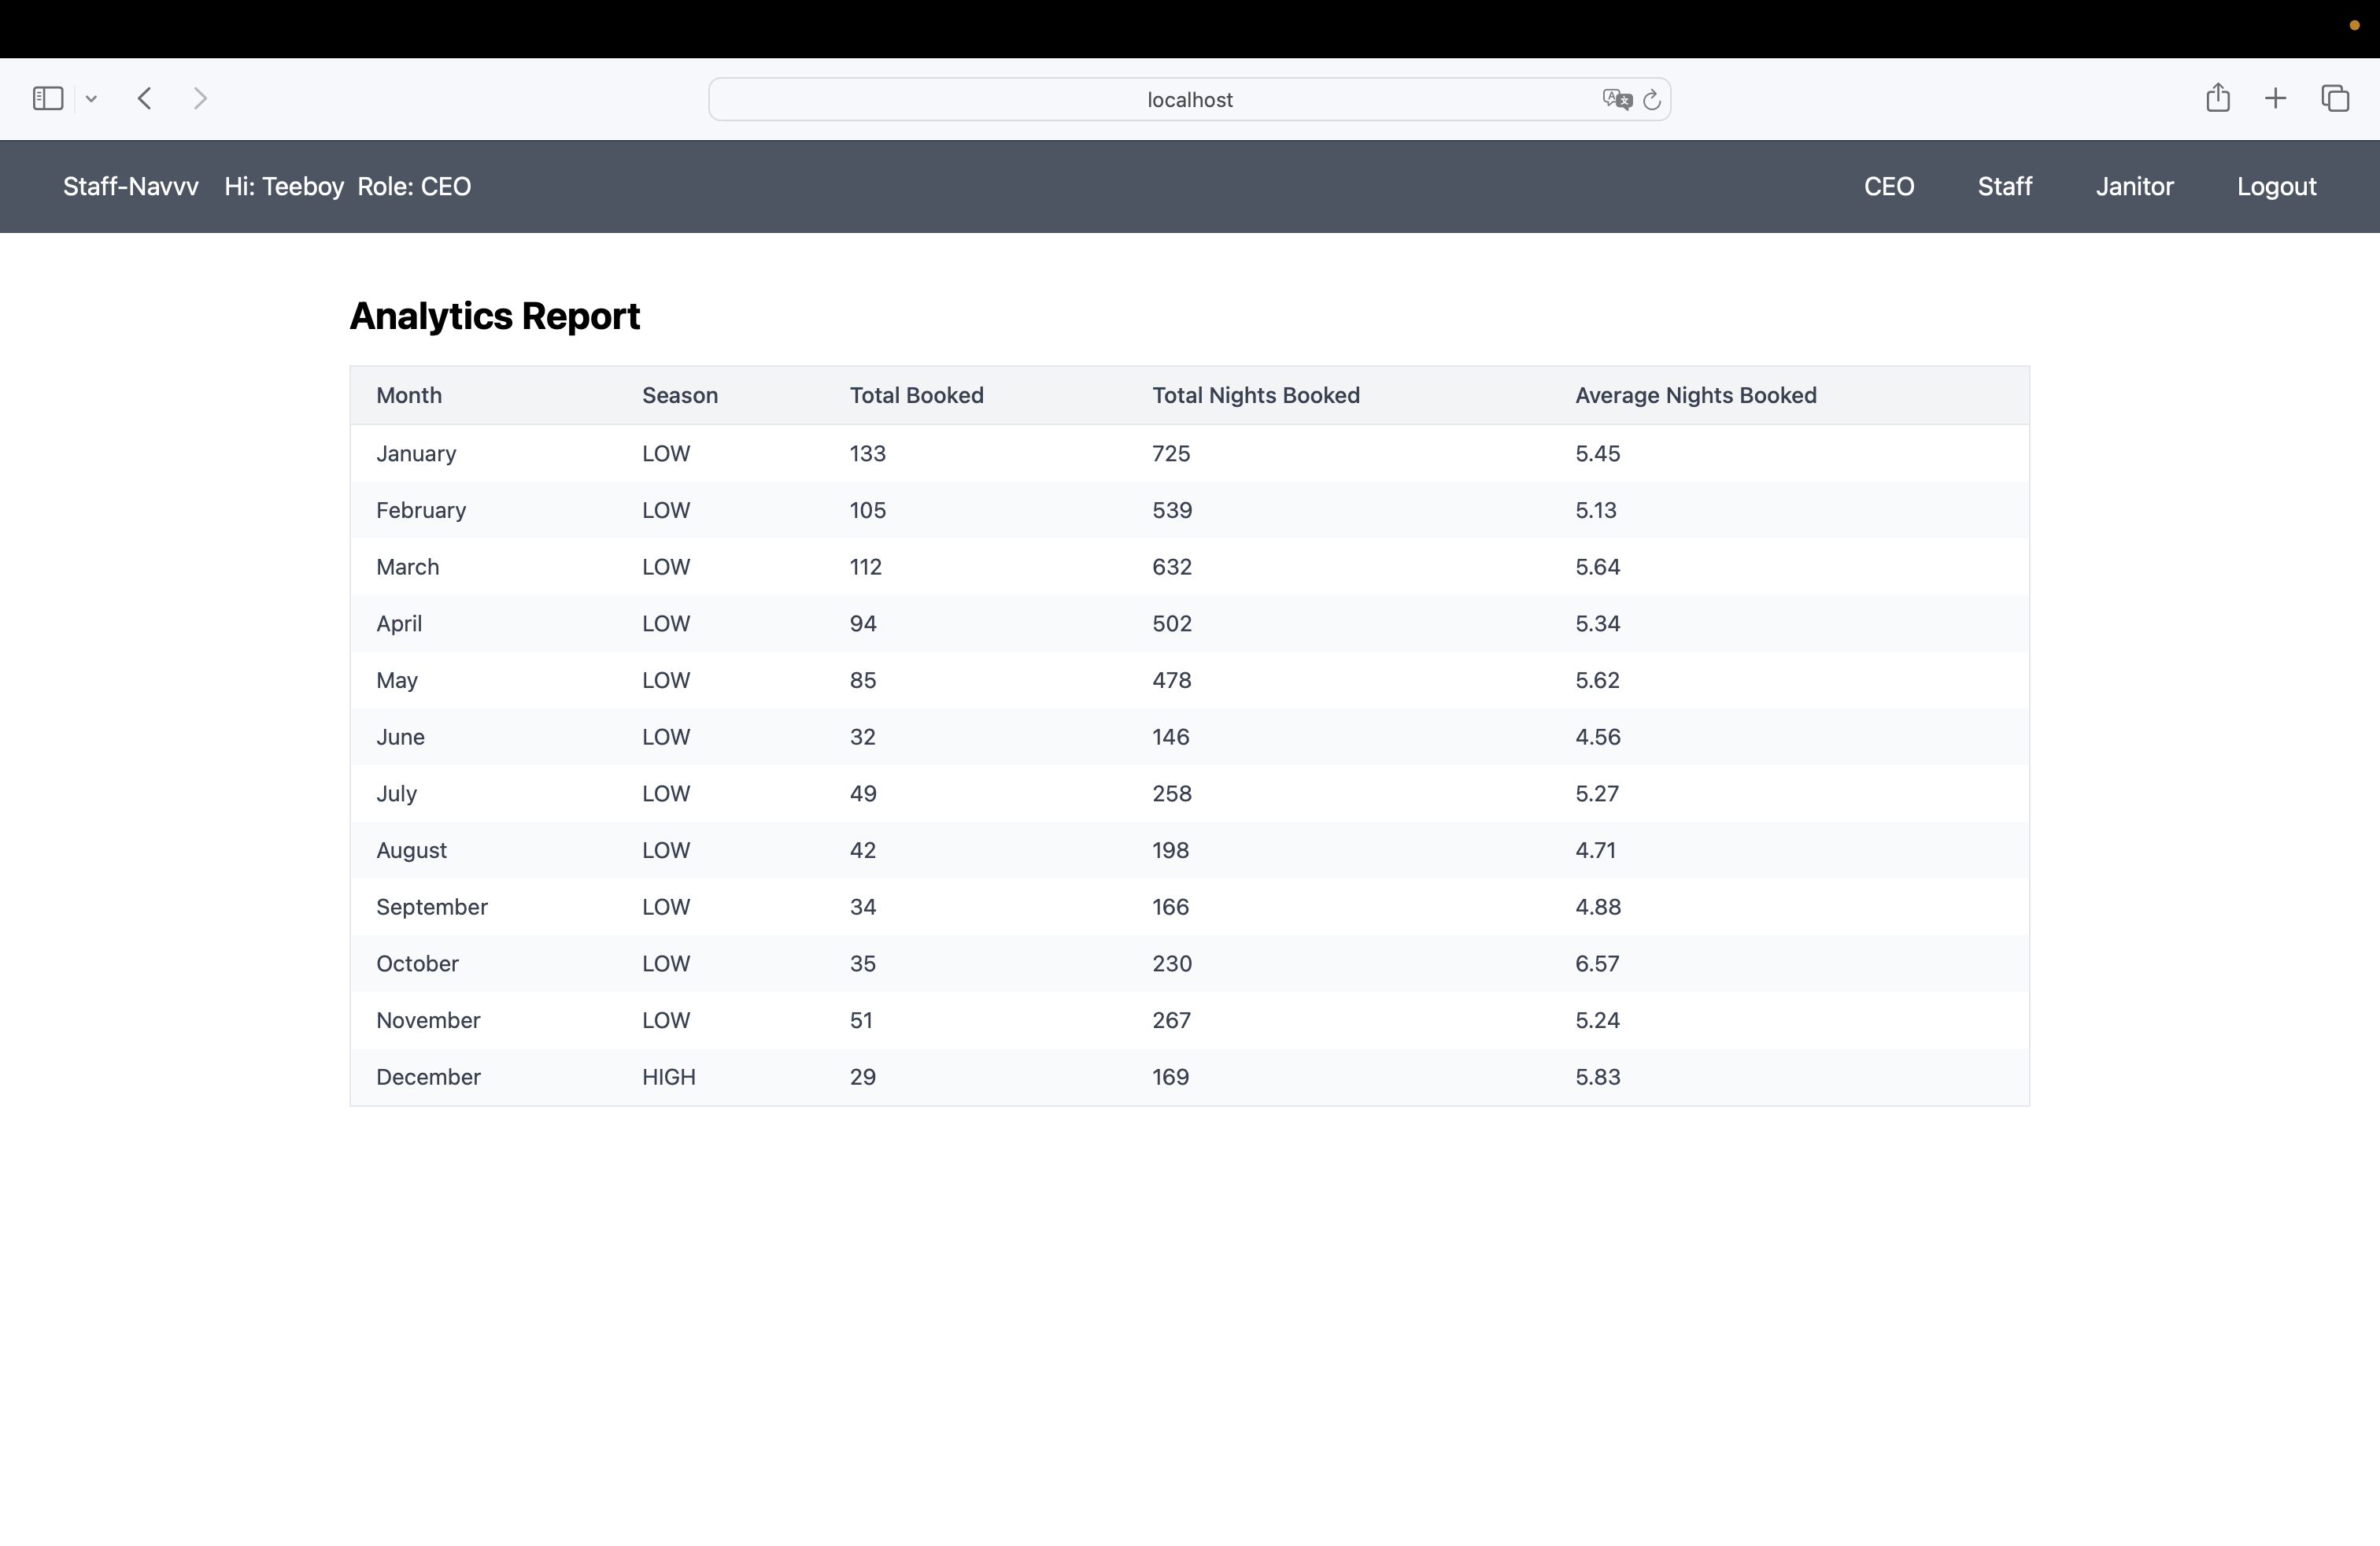
\includegraphics[width=12cm]{fig/5_summary}}
	%{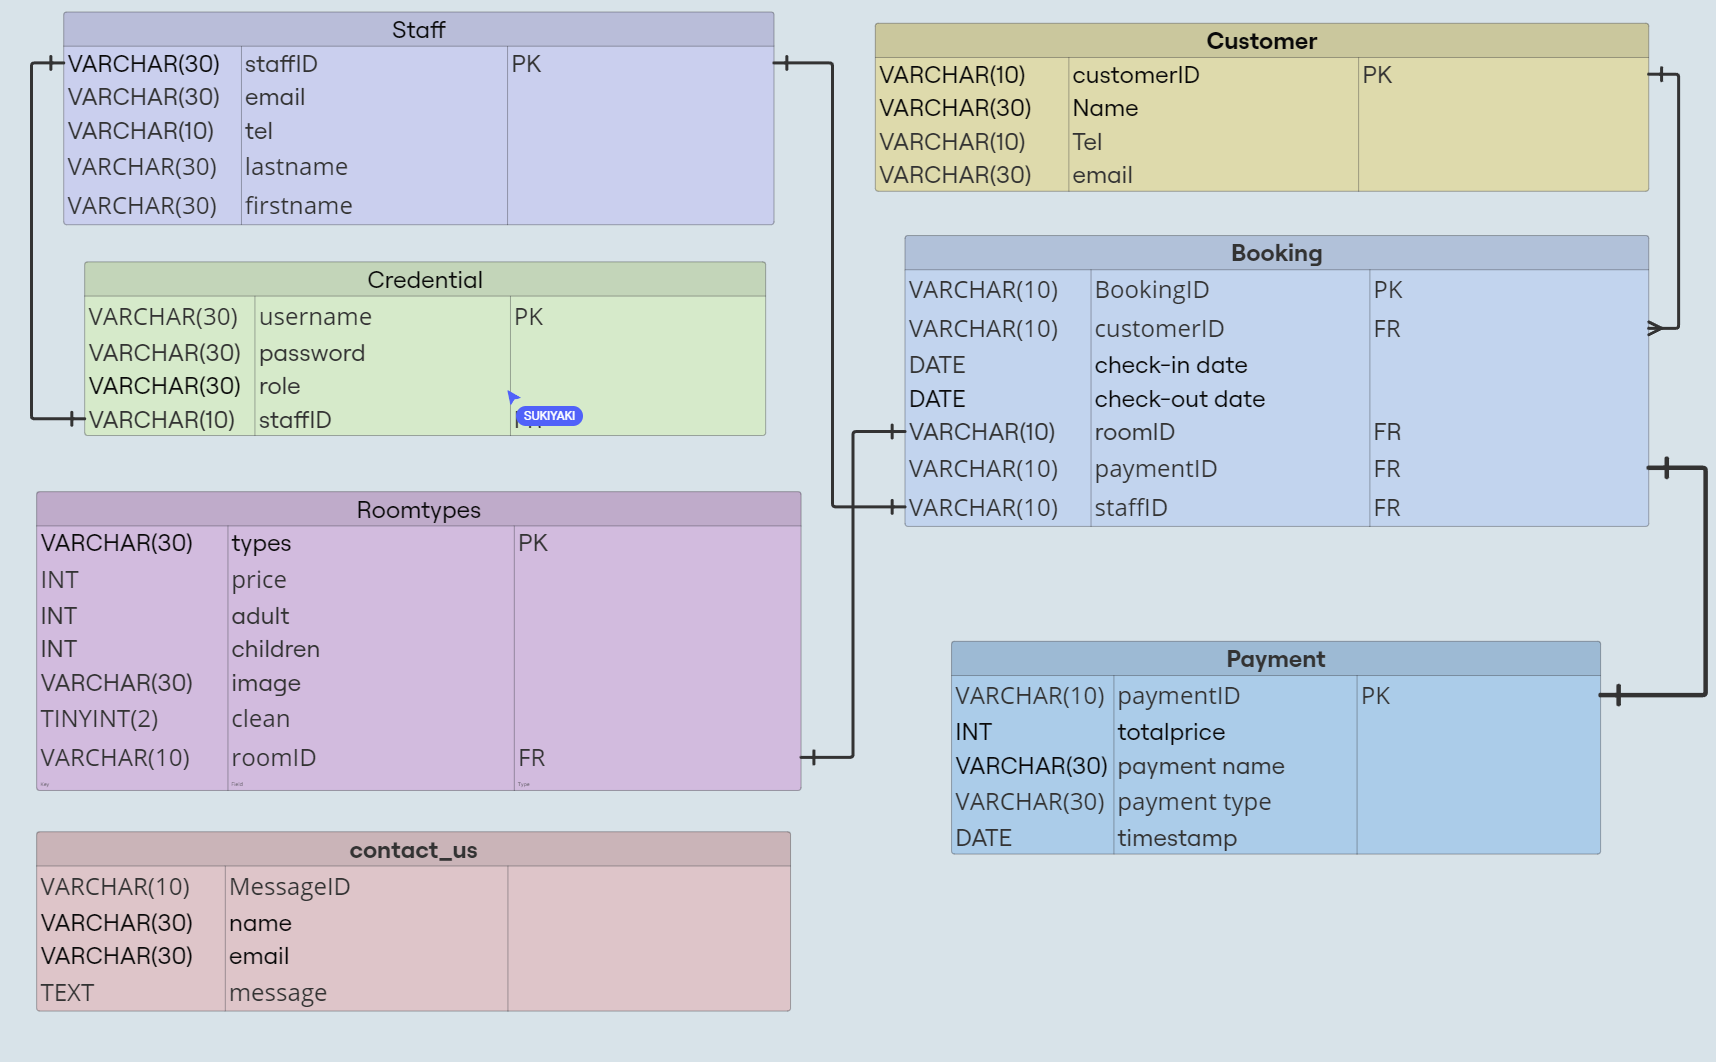
\includegraphics[]{fig/ERD_v1}}
	\caption{Summary report}
\end{figure} 

Relations involved: Invoice, Seasons Discount, Reservations

\subsection{Company Report}
\begin{figure}[h]
	\centerline
	{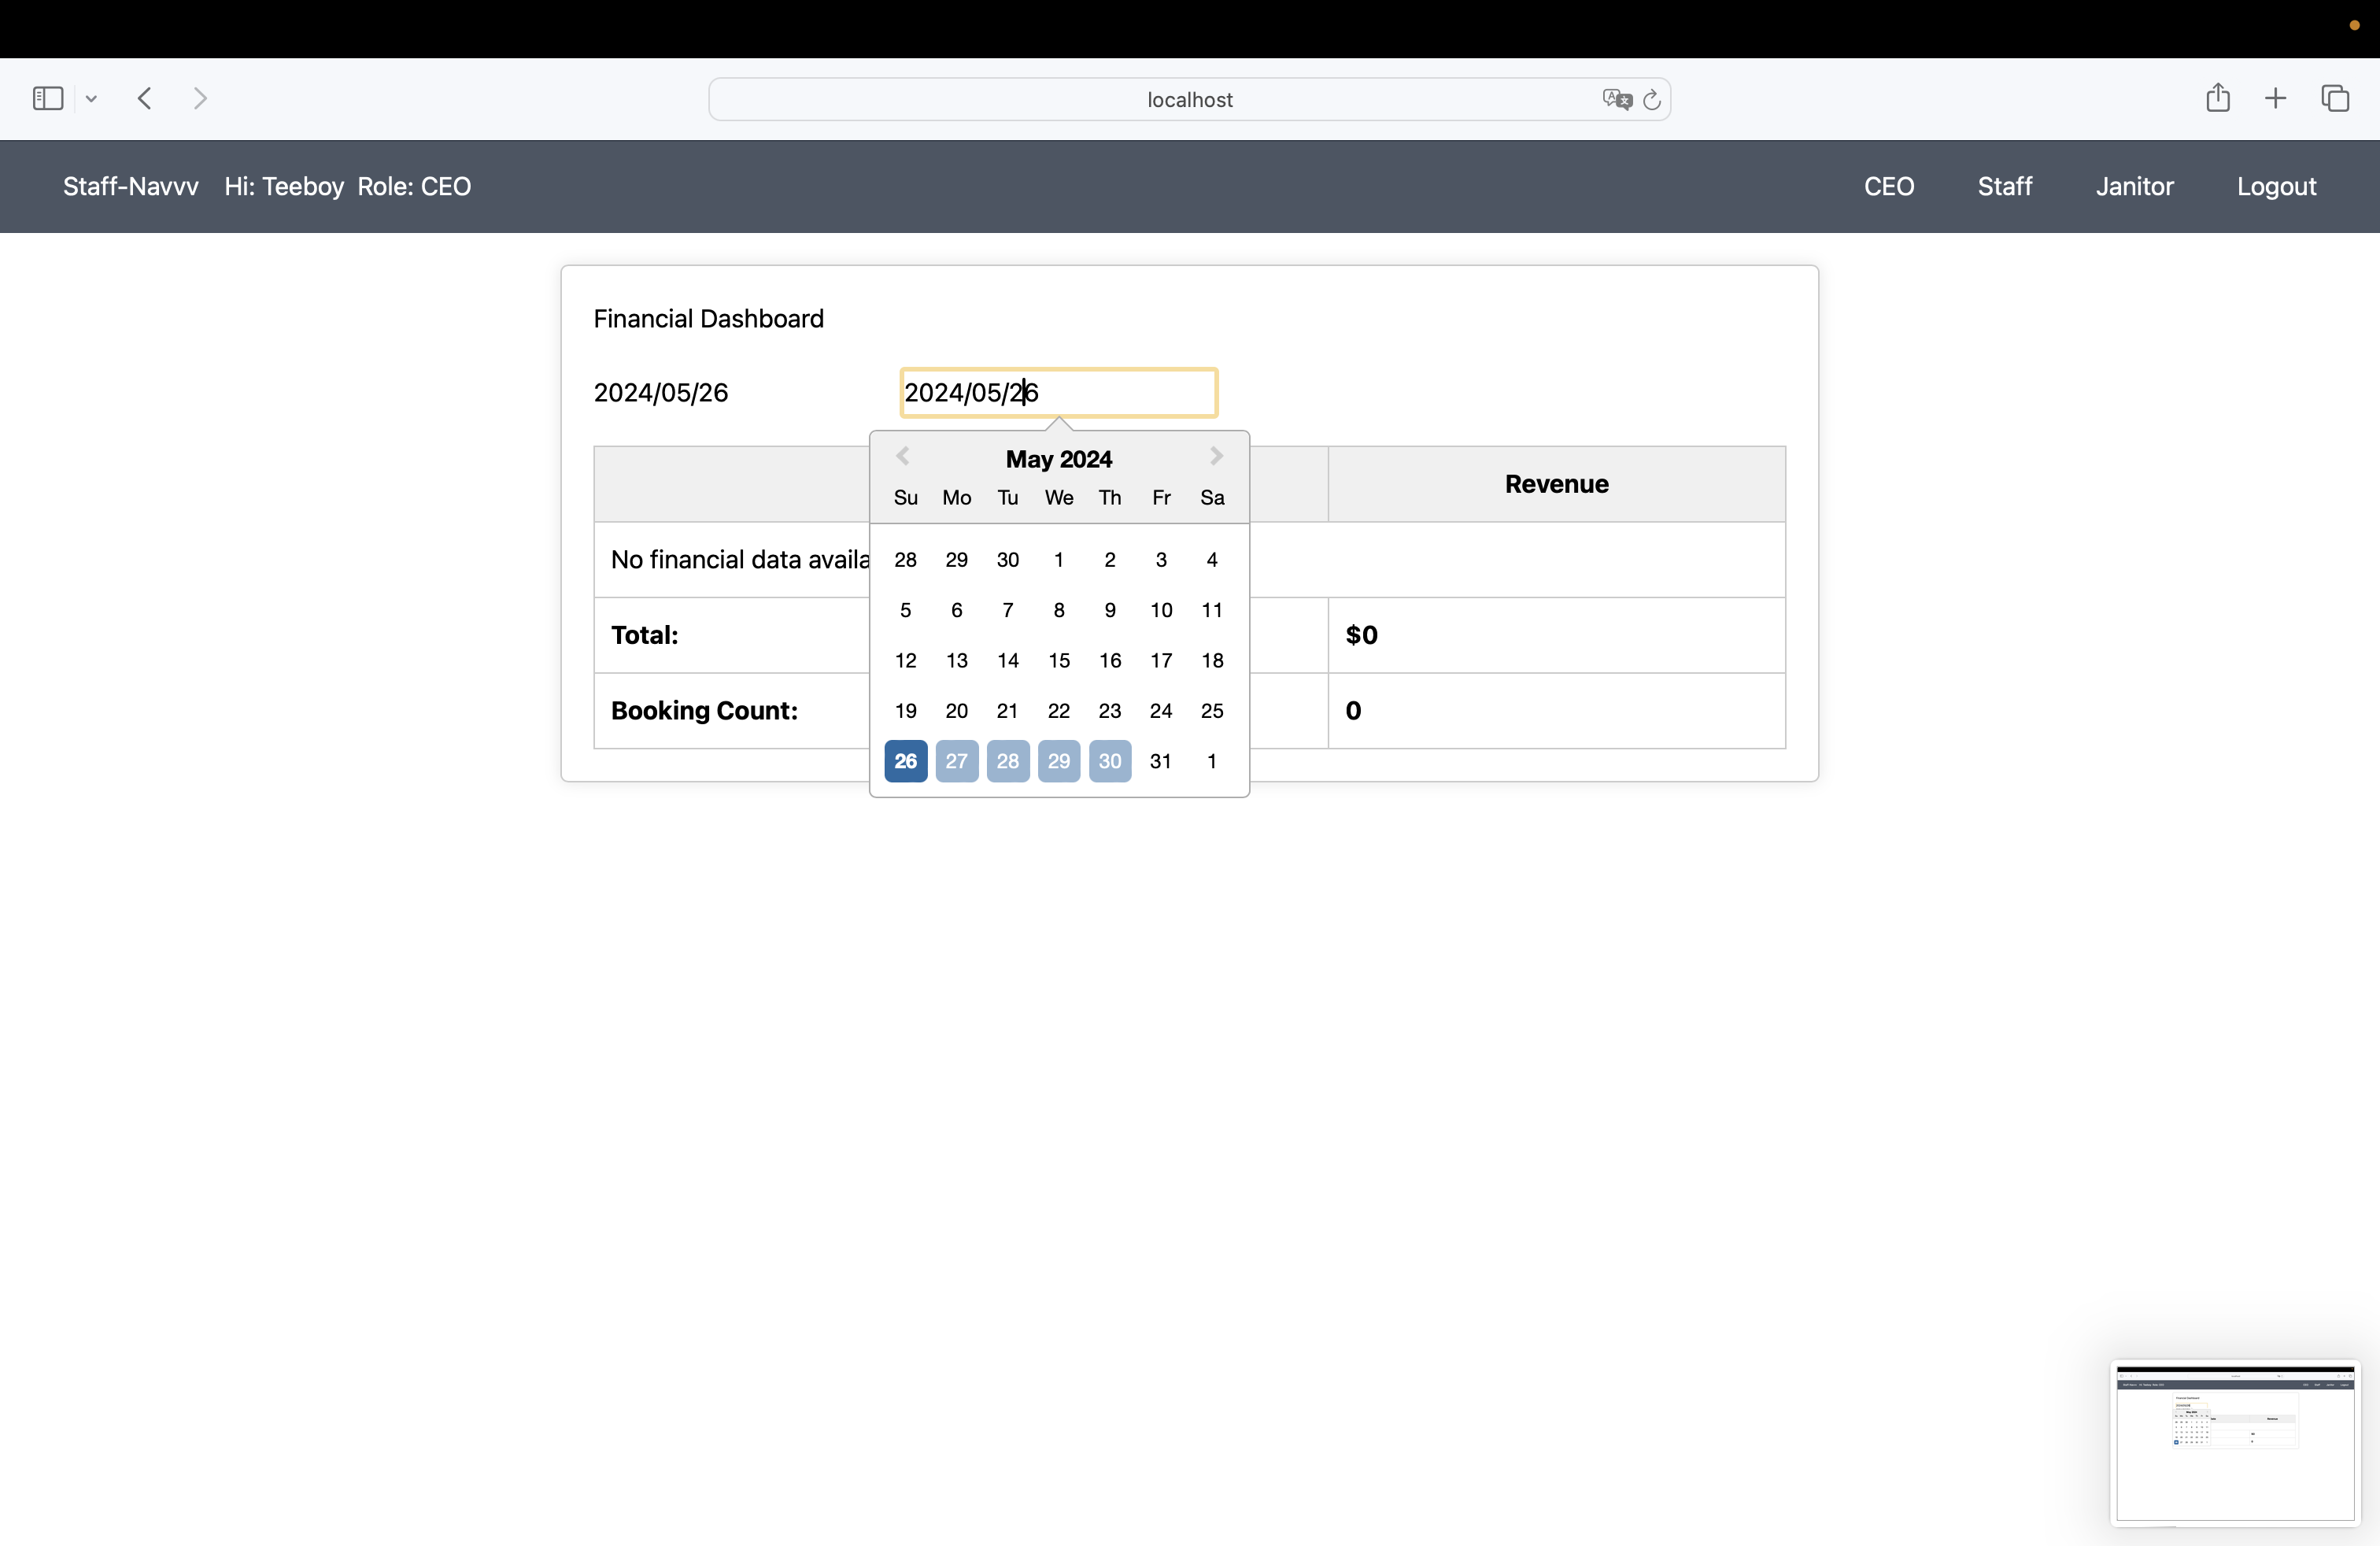
\includegraphics[width=12cm]{fig/6_company}}
	%{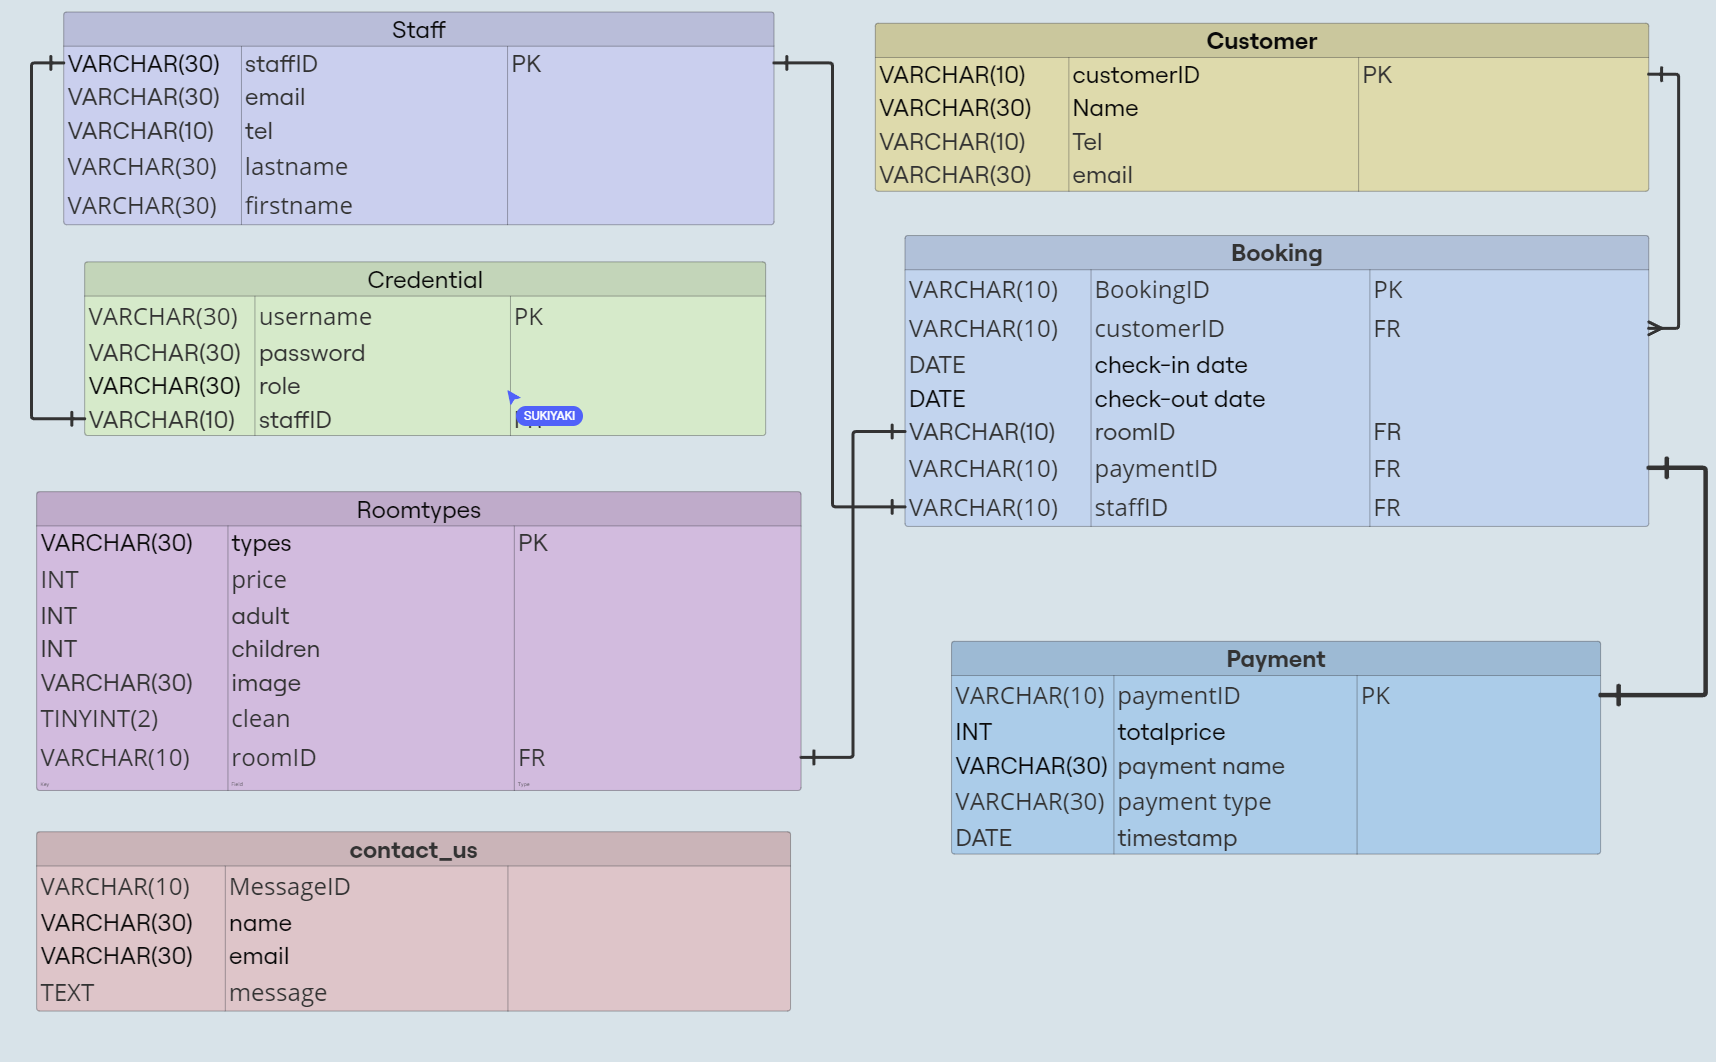
\includegraphics[]{fig/ERD_v1}}
	\caption{Company report}
\end{figure} 

Relations involved: Invoice, Seasons Discount

Viewing invoice against seasons discount allows us to see the correlation between revenue when the discount is provided.

\clearpage
%=========================================================